% Provenance (never printed): cycle 3 "La planete Terre" and geography
% (weather and climate; reading a climate chart; the great climate zones of
% the world, hot, temperate and cold); see sources/book1/PROVENANCE.md.
% Book 1, grade 5, chapter 2.
\chapter{El tiempo y el clima}\label{ch:g5:weather-and-climate}

En la segunda semana de enero llegan dos postales al colegio. La primera,
de la prima de Lena, muestra a unos niños haciendo un castillo de \omterm{def:g3:stones-pebbles-sand:sand}{arena} en
una playa soleada, bajo las palmeras. La segunda, de la abuela de Tom,
muestra a unos niños haciendo un muñeco de \omterm{def:g4:clouds-rain-snow:precipitation}{nieve} en un jardín nevado.
---¿Cómo puede ser verano e invierno en la misma semana? ---pregunta Tom.

Lo que tanto cambia de un lugar a otro no es el \omterm{def:g1:watching-the-weather:weather}{tiempo} de un día. Es el
\omterm{def:g1:watching-the-weather:weather}{tiempo} que tienen año tras año: su \omterm{def:g5:weather-and-climate:climate}{clima}.

\begin{omfigure}
\begin{minipage}[b]{0.48\linewidth}\centering

\includegraphics[width=\linewidth]{images/book1/ai/g5-beach-postcard.jpg}
\end{minipage}\hfill
\begin{minipage}[b]{0.48\linewidth}\centering

\includegraphics[width=\linewidth]{images/book1/ai/g5-snowman-postcard.jpg}
\end{minipage}

{\small Dos postales de la misma semana de enero: una playa soleada y un
jardín nevado.}
\end{omfigure}

\begin{recall}
El \omterm{def:g1:watching-the-weather:weather}{tiempo} es el estado del aire en un lugar y un momento dados: soleado,
nublado, lluvioso, nevoso, ventoso (\cref{ch:g1:watching-the-weather}). Un
termómetro mide la temperatura del aire, en grados Celsius; un \omterm{def:g4:clouds-rain-snow:rain-gauge}{pluviómetro}
mide la \omterm{def:g4:clouds-rain-snow:precipitation}{lluvia}, en milímetros (\cref{ch:g4:clouds-rain-snow}). El \omterm{def:g3:continents-and-oceans:equator}{ecuador}
da la vuelta al \omterm{def:g3:continents-and-oceans:globe}{globo} por el medio, a mitad de camino entre el \omterm{def:g3:continents-and-oceans:poles}{Polo Norte} y
el \omterm{def:g3:continents-and-oceans:poles}{Polo Sur} (\cref{ch:g3:continents-and-oceans}). Los libros de física
mostraron que la Tierra da una vuelta alrededor del Sol en un año, y que sus
estaciones se deben a la inclinación de su eje: en verano, el Sol sube más
alto en el cielo y los días son más largos.
\end{recall}

\section{El tiempo es el de hoy; el clima, el de siempre}

El \omterm{def:g1:watching-the-weather:weather}{tiempo} cambia de un día para otro, e incluso de una hora a otra. El
\omterm{def:g5:weather-and-climate:climate}{clima} es otra cosa.

\begin{definition}[Clima]\label{def:g5:weather-and-climate:climate}
El \emph{clima}\index{clima} de un lugar es el \omterm{def:g1:watching-the-weather:weather}{tiempo} que hace allí
normalmente, mes a mes, a lo largo de muchos años: lo cálida o fría, lo
húmeda o seca que es cada estación. Los científicos del \omterm{def:g1:watching-the-weather:weather}{tiempo} lo calculan
haciendo la media de las mediciones de 30 años.
% ledger: wmo:normal-30yr
\end{definition}

``Esta mañana llueve'' es una frase sobre el \omterm{def:g1:watching-the-weather:weather}{tiempo}. ``Aquí llueve mucho en
otoño'' es una frase sobre el \omterm{def:g5:weather-and-climate:climate}{clima}. Un solo día frío en verano no cambia
el \omterm{def:g5:weather-and-climate:climate}{clima}; es solo un \omterm{def:g1:watching-the-weather:weather}{tiempo} poco habitual.

Los científicos del \omterm{def:g1:watching-the-weather:weather}{tiempo} de todo el mundo siguen la misma regla: hacen la
media de 30 años de mediciones. Las medias que se usan hoy son las de los
años 1991 a 2020.
% ledger: wmo:normal-30yr

\section{El climograma}

Para mostrar el \omterm{def:g5:weather-and-climate:climate}{clima} de un lugar en una sola imagen, dibujamos un gráfico.

\begin{definition}[Climograma]\label{def:g5:weather-and-climate:climate-chart}
Un \emph{climograma}\index{climograma} muestra, para cada mes del año, la
temperatura media de un lugar (una curva) y la cantidad media de \omterm{def:g4:clouds-rain-snow:precipitation}{lluvia} y
\omterm{def:g4:clouds-rain-snow:precipitation}{nieve} que cae en él (barras, en milímetros de agua).
\end{definition}

\begin{omfigure}
\begin{tikzpicture}
  \begin{axis}[name=pax, width=0.55\linewidth, height=5.6cm, ymin=0, ymax=400,
      axis y line*=right, axis x line=none, ybar, bar width=7pt,
      ytick={0,100,...,400}, ylabel={lluvia (mm)}, xmin=0.4, xmax=12.6,
      tick label style={font=\scriptsize}, label style={font=\scriptsize},
      ylabel style={blue!60!black}]
    \addplot[fill=blue!40, draw=blue!60!black]
      table[x=month, y=prcp_mm] {figdata/out/grade-5-climate_charts-seattle.dat};
  \end{axis}
  \begin{axis}[width=0.55\linewidth, height=5.6cm, ymin=-30, ymax=40,
      axis y line*=left, axis x line*=bottom, xmin=0.4, xmax=12.6,
      xtick={1,...,12}, xticklabels={E,F,M,A,M,J,J,A,S,O,N,D},
      ytick={-30,-20,...,40}, ylabel={temperatura ($^\circ$C)},
      tick label style={font=\scriptsize}, label style={font=\scriptsize},
      ylabel style={red!70!black}]
    \addplot[red!70!black, thick, mark=*, mark size=1.3pt]
      table[x=month, y=tavg_C] {figdata/out/grade-5-climate_charts-seattle.dat};
    \draw[gray!60] (axis cs:0.4,0) -- (axis cs:12.6,0);
    \begin{scope}[every node/.style={circle, draw, fill=white, inner sep=0.8pt,
        font=\scriptsize\bfseries}]
      \node[text=red!70!black, draw=red!70!black] at (axis cs:5.5,27) {1};
      \node[text=blue!60!black, draw=blue!60!black] at (axis cs:7,-19) {2};
    \end{scope}
  \end{axis}
  \node[anchor=north west, font=\scriptsize, align=left, text width=4.2cm]
    at ($(pax.outer north east)+(0.3,-0.1)$) {%
    \textcolor{red!70!black}{\textbf{1} La curva roja: la temperatura media
    de cada mes, que se lee en la escala de la izquierda.}\par\smallskip
    \textcolor{blue!60!black}{\textbf{2} Las barras azules: la lluvia media de
    cada mes, que se lee en la escala de la derecha.}\par\smallskip
    \textbf{3} Las letras bajo el gráfico: los meses, de enero a
    diciembre.};
\end{tikzpicture}

{\small El \omterm{def:g5:weather-and-climate:climate-chart}{climograma} de Seattle, una ciudad de la \omterm{def:g1:landscapes-around-us:water}{costa} oeste de los
Estados Unidos. Medias de los años 1991 a 2020 (datos: NOAA).}
% ledger: data:b1-noaa-normals
\end{omfigure}

\begin{method}[Leer un climograma]\label{met:g5:weather-and-climate:reading}
\begin{enumerate}
  \item Busca el mes más cálido y el más frío en la curva roja, y lee sus
        temperaturas en la escala de la izquierda. ¿La curva es plana (la
        misma temperatura todo el año) o sube y baja (estaciones cálidas y
        frías)? ¿Baja de 0~$^\circ$C (helada)?
  \item Busca el mes más lluvioso y el más seco entre las barras azules, y
        léelos en la escala de la derecha. ¿Las barras son altas o bajas?
        ¿Hay una estación seca?
  \item Resúmelo en una frase: ``cálido y seco todo el año'', ``suave y
        lluvioso, con un verano seco''{\ldots}
\end{enumerate}
\end{method}

\begin{example}[Seattle]\label{ex:g5:weather-and-climate:seattle}
En Seattle, el mes más cálido es agosto (unos 20~$^\circ$C) y el más frío
es diciembre (unos 6~$^\circ$C): la curva sube y baja, pero nunca baja de
cero. La barra más alta es la de noviembre (unos 160~mm), y la más baja, la
de julio (unos 15~mm). En una frase: inviernos suaves, veranos frescos,
lluvioso en otoño y en invierno, más bien seco en verano. En un año entero
caen unos 1\,000~milímetros de \omterm{def:g4:clouds-rain-snow:precipitation}{lluvia}: un metro de agua.
% ledger: data:b1-noaa-normals
\end{example}

\section{Cuatro climas}

Aquí tienes los \omterm{def:g5:weather-and-climate:climate-chart}{climogramas} de cuatro ciudades de los Estados Unidos, muy
alejadas entre sí: Phoenix, en el \omterm{def:g5:weather-and-climate:desert}{desierto} de Arizona; Hilo, en la isla de
Hawái, en medio del \omterm{def:g2:water-on-earth:ocean}{océano} Pacífico; Seattle, en la \omterm{def:g1:landscapes-around-us:water}{costa} oeste; y
Utqiaġvik, en el extremo norte de Alaska, a orillas del \omterm{def:g2:water-on-earth:ocean}{océano} Ártico. Los
cuatro gráficos usan las mismas escalas, así que podemos compararlos de un
vistazo.

\begin{omfigure}
\def\gfivechart#1#2{%
\begin{tikzpicture}
  \begin{axis}[width=0.5\linewidth, height=4.6cm, ymin=0, ymax=400,
      axis y line*=right, axis x line=none, ybar, bar width=4pt,
      ytick={0,100,...,400}, xmin=0.4, xmax=12.6,
      tick label style={font=\tiny}]
    \addplot[fill=blue!40, draw=blue!60!black]
      table[x=month, y=prcp_mm] {figdata/out/grade-5-climate_charts-#1.dat};
  \end{axis}
  \begin{axis}[width=0.5\linewidth, height=4.6cm, ymin=-30, ymax=40,
      axis y line*=left, axis x line*=bottom, xmin=0.4, xmax=12.6,
      xtick={1,...,12}, xticklabels={E,F,M,A,M,J,J,A,S,O,N,D},
      ytick={-30,-20,...,40}, tick label style={font=\tiny},
      title={#2}, title style={font=\scriptsize\bfseries, yshift=-4pt}]
    \addplot[red!70!black, thick, mark=*, mark size=1pt]
      table[x=month, y=tavg_C] {figdata/out/grade-5-climate_charts-#1.dat};
    \draw[gray!60] (axis cs:0.4,0) -- (axis cs:12.6,0);
  \end{axis}
\end{tikzpicture}}%
\gfivechart{phoenix}{Phoenix: un \omterm{def:g5:weather-and-climate:desert}{desierto} cálido}\hfill
\gfivechart{hilo}{Hilo: un \omterm{def:g5:weather-and-climate:climate}{clima} de \omterm{def:g5:weather-and-climate:rainforest}{selva tropical}}

\medskip
\gfivechart{seattle}{Seattle: un \omterm{def:g5:weather-and-climate:climate}{clima} templado}\hfill
\gfivechart{utqiagvik}{Utqiaġvik: un \omterm{def:g5:weather-and-climate:climate}{clima} polar}

{\small Cuatro \omterm{def:g5:weather-and-climate:climate-chart}{climogramas} con las mismas escalas: la temperatura en
$^\circ$C a la izquierda (curva roja) y la \omterm{def:g4:clouds-rain-snow:precipitation}{lluvia} en milímetros a la derecha
(barras azules). Medias de los años 1991 a 2020 (datos: NOAA).}
% ledger: data:b1-noaa-normals
\end{omfigure}

\paragraph{El desierto.} En Phoenix, las barras son tan bajas que apenas se
ven: en un año entero caen menos de 200 milímetros de \omterm{def:g4:clouds-rain-snow:precipitation}{lluvia}. Los veranos
son muy calurosos: en julio la temperatura media es de 35 grados.
% ledger: data:b1-noaa-normals

\begin{definition}[Desierto]\label{def:g5:weather-and-climate:desert}
Un \emph{desierto}\index{desierto} es un lugar donde cae muy poca \omterm{def:g4:clouds-rain-snow:precipitation}{lluvia}:
menos de 250 milímetros al año. Pocas plantas pueden vivir en él, y el
suelo suele estar desnudo.
% ledger: usgs:arid-250mm
\end{definition}

Los \omterm{def:g5:weather-and-climate:desert}{desiertos} no siempre son cálidos. Fíjate en Utqiaġvik: allí caen menos
de 150 milímetros al año, aún menos que en Phoenix; es un \omterm{def:g5:weather-and-climate:desert}{desierto} frío.
Los \omterm{def:g5:weather-and-climate:desert}{desiertos} pueden ser cálidos o fríos.
% ledger: data:b1-noaa-normals, usgs:arid-250mm

\paragraph{La selva tropical.} Hilo es lo contrario de Phoenix. Sus barras
son las más altas de los cuatro gráficos: caen más de 3\,000 milímetros de
\omterm{def:g4:clouds-rain-snow:precipitation}{lluvia} al año, y todos los meses son lluviosos. Y su curva roja es casi
plana: entre 22 y 25 grados todo el año. No hay invierno en absoluto.
% ledger: data:b1-noaa-normals

\begin{definition}[Selva tropical]\label{def:g5:weather-and-climate:rainforest}
Una \emph{selva tropical}\index{selva tropical} es un bosque espeso de
árboles muy altos que crece donde hace calor y hay humedad todo el año, con
\omterm{def:g4:clouds-rain-snow:precipitation}{lluvias} fuertes todos los meses. La mayoría de las selvas tropicales están
cerca del \omterm{def:g3:continents-and-oceans:equator}{ecuador}.
\end{definition}

\begin{omfigure}
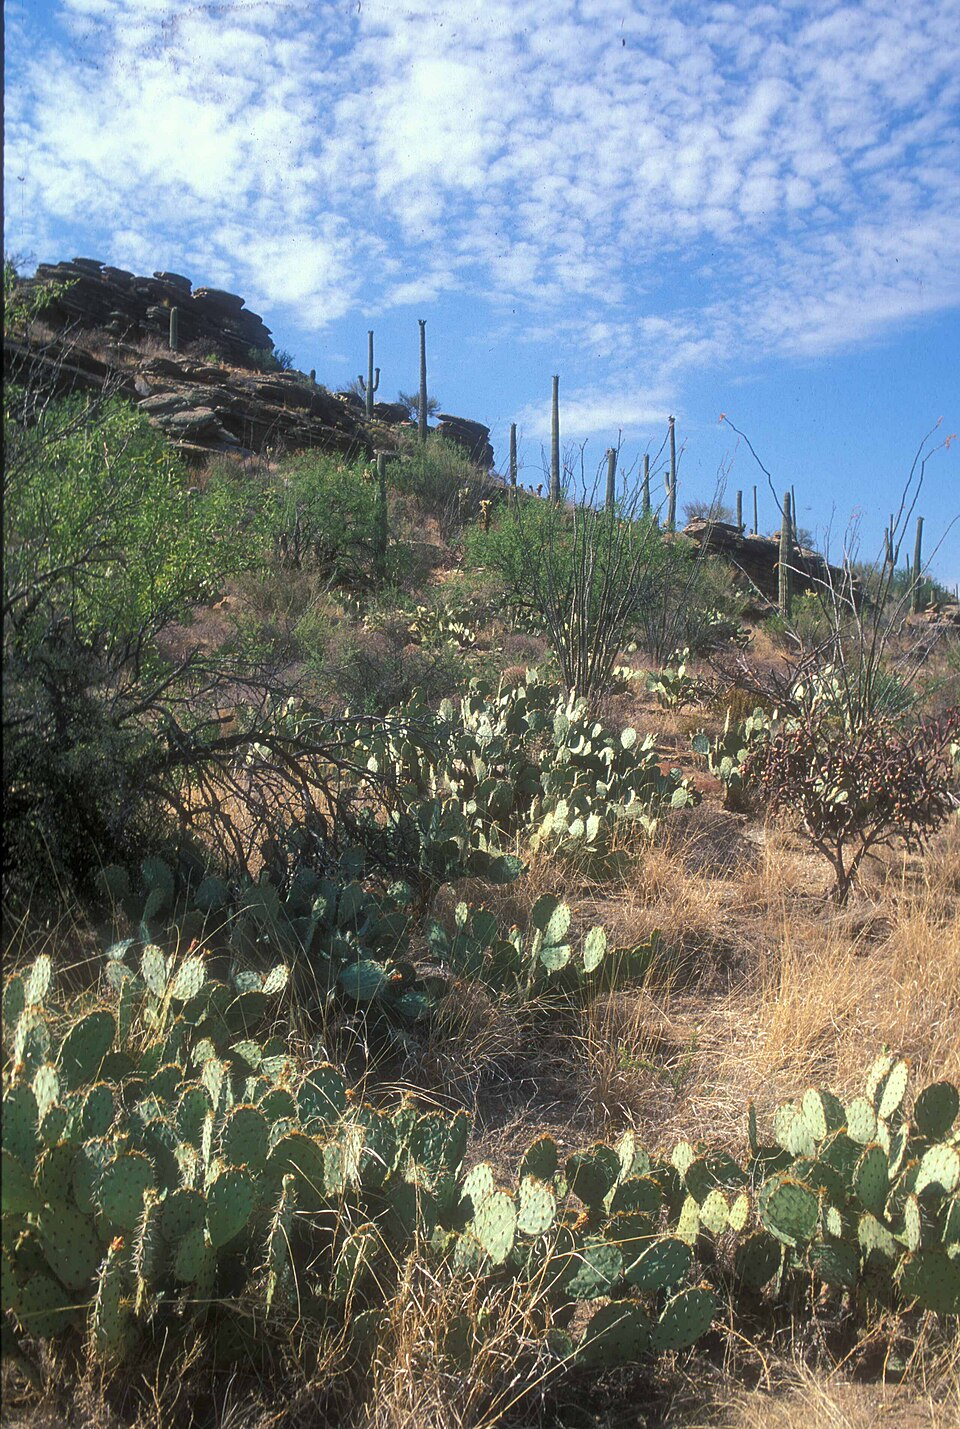
\includegraphics[height=3.6cm]{images/book1/g5-sonoran-desert.jpg}\quad
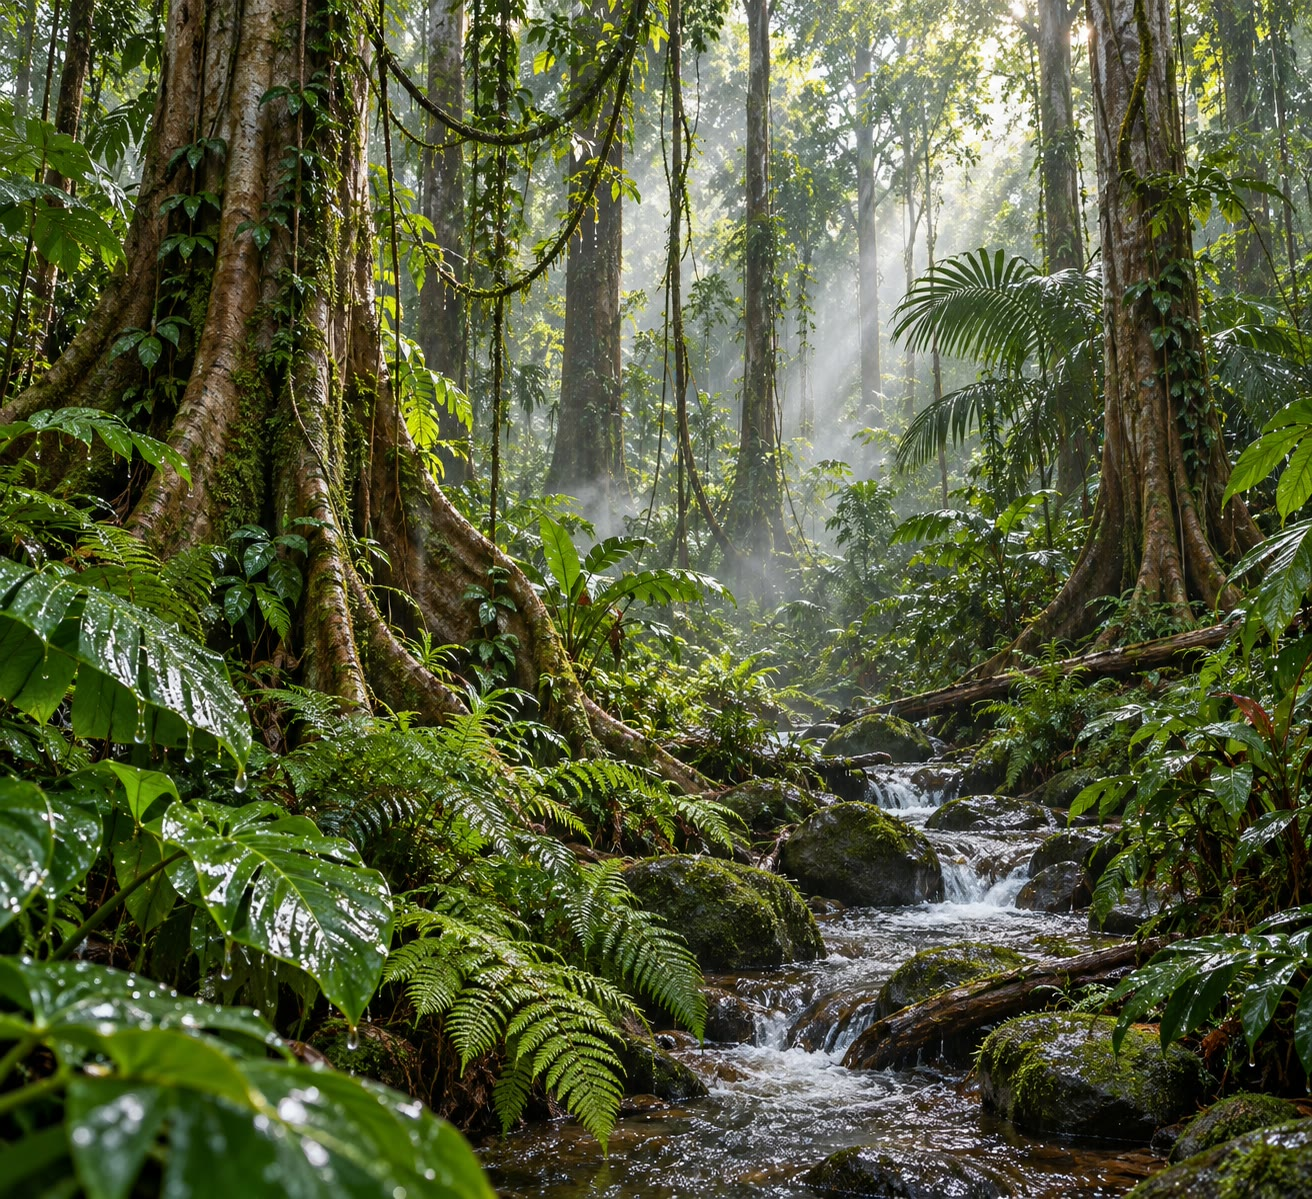
\includegraphics[height=3.6cm]{images/book1/ai/g5-rainforest.jpg}\quad
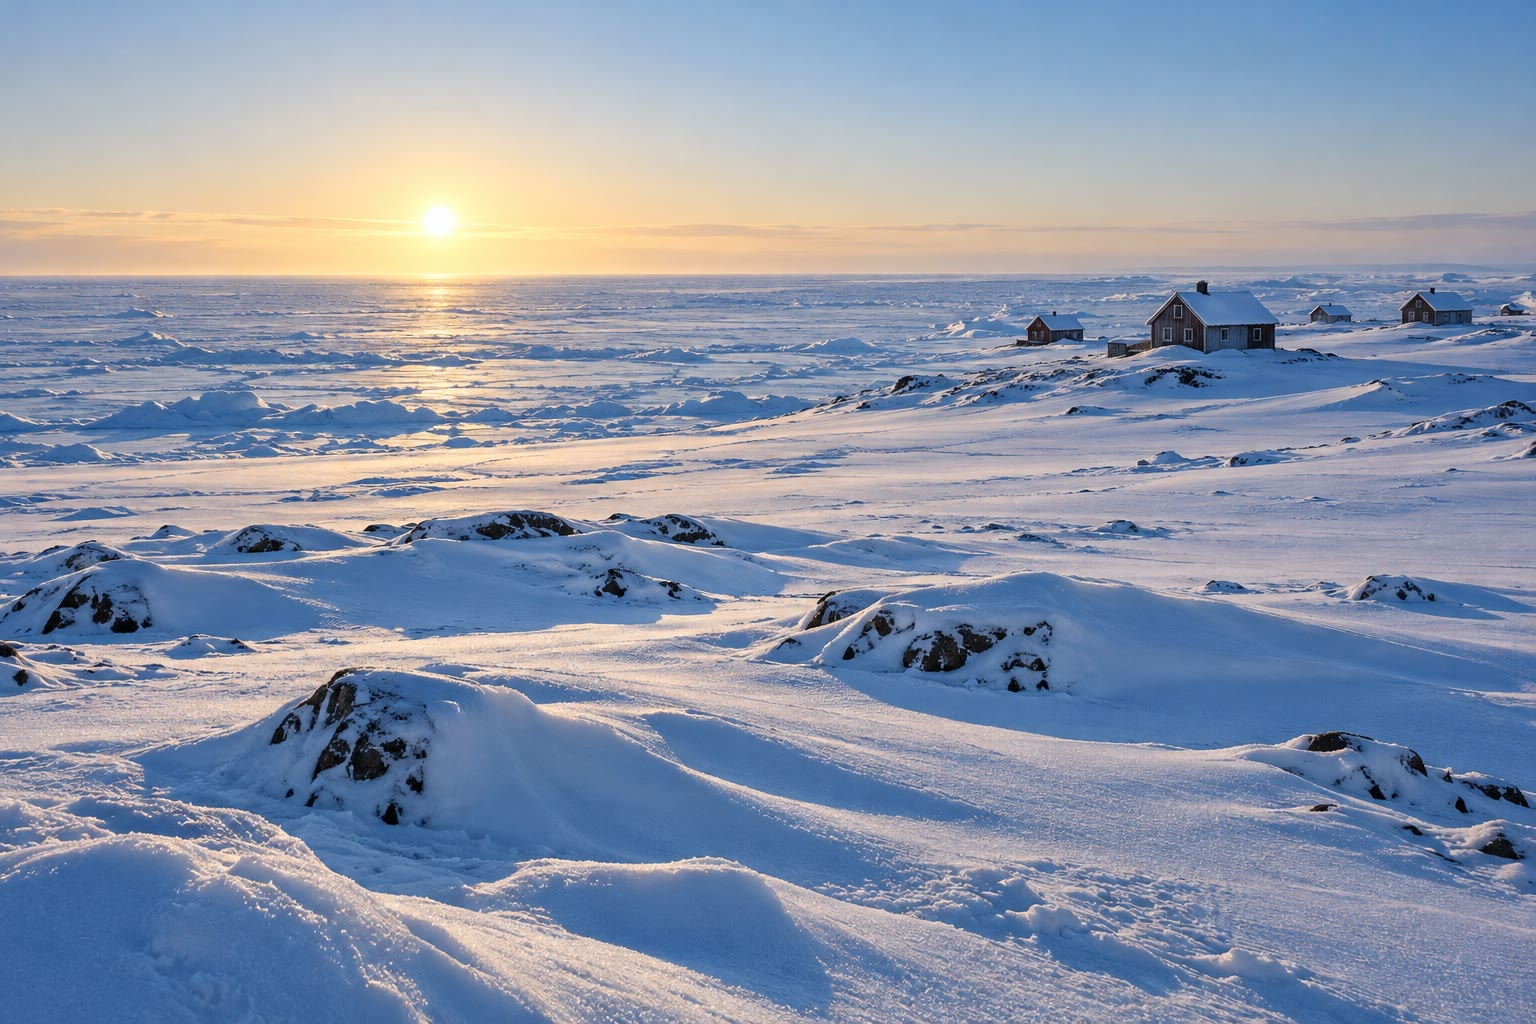
\includegraphics[height=3.6cm]{images/book1/ai/g5-polar-tundra.jpg}

{\small Tres \omterm{def:g5:weather-and-climate:climate}{climas} extremos. A la izquierda, el \omterm{def:g5:weather-and-climate:desert}{desierto} de Sonora, en
Arizona, el \omterm{def:g5:weather-and-climate:desert}{desierto} de Phoenix, con altos cactus saguaros y chumberas, que
guardan agua en sus tallos gruesos (fotografía: U.S. National Park Service,
Saguaro National Park, dominio público). En el centro, el interior de una
\omterm{def:g5:weather-and-climate:rainforest}{selva tropical} después de un chaparrón. A la derecha, una \omterm{def:g1:landscapes-around-us:water}{costa} polar en
invierno, con el \omterm{def:g2:water-on-earth:ocean}{mar} helado y el Sol bajo a mediodía.}
% ledger: nps:sonoran-desert
\end{omfigure}

\paragraph{El clima templado.} Seattle está entre los dos: su curva sube en
verano y baja en invierno, pero nunca mucho; llueve bastante, sobre todo en
otoño y en invierno. Es un \omterm{def:g5:weather-and-climate:climate}{clima} templado: ni grandes calores ni grandes
fríos.

\paragraph{El clima polar.} En Utqiaġvik, la curva roja se queda por debajo
de 0~$^\circ$C ocho meses al año; en febrero la media es de 24 grados bajo
cero. Incluso en julio, el mes más cálido, solo hay unos 5 grados.
% ledger: data:b1-noaa-normals

\section{Zonas cálida, templadas y frías}

¿Por qué hace calor cerca del \omterm{def:g3:continents-and-oceans:equator}{ecuador} y frío cerca de los \omterm{def:g3:continents-and-oceans:poles}{polos}? Por el
Sol. Cerca del \omterm{def:g3:continents-and-oceans:equator}{ecuador}, el Sol del mediodía está alto en el cielo todo el
año: su luz cae casi en vertical y calienta mucho el suelo. Cerca de los
\omterm{def:g3:continents-and-oceans:poles}{polos}, el Sol se queda siempre bajo: su luz llega inclinada, repartida
sobre una gran superficie, y calienta poco. Allí, en invierno, puede que el
Sol ni siquiera salga.

Dos pares de líneas alrededor del \omterm{def:g3:continents-and-oceans:globe}{globo} dividen la Tierra en \omterm{def:g5:weather-and-climate:climate-zone}{zonas climáticas}.

\begin{definition}[Trópicos y círculos polares]\label{def:g5:weather-and-climate:tropics}
Los dos \emph{trópicos}\index{tropico@trópico} son las líneas que dan la
vuelta al \omterm{def:g3:continents-and-oceans:globe}{globo}, una al norte y otra al sur del \omterm{def:g3:continents-and-oceans:equator}{ecuador}, que marcan hasta
qué distancia del \omterm{def:g3:continents-and-oceans:equator}{ecuador} puede estar el Sol del mediodía justo en lo alto:
el trópico de Cáncer al norte y el trópico de Capricornio al sur. Los dos
\emph{círculos polares}\index{circulo polar@círculo polar} son las líneas
que dan la vuelta al \omterm{def:g3:continents-and-oceans:globe}{globo}, cerca de los \omterm{def:g3:continents-and-oceans:poles}{polos}, más allá de las cuales, en
pleno invierno, el Sol no sale durante al menos un día, y en pleno verano
no se pone: el círculo polar ártico al norte y el círculo polar antártico
al sur.
\end{definition}

La inclinación del eje de la Tierra decide dónde están esas líneas.

\begin{definition}[Zonas climáticas]\label{def:g5:weather-and-climate:climate-zone}
La Tierra se divide en tres clases de \emph{zona climática}\index{zona climatica@zona climática}: la \emph{zona cálida}, entre los dos \omterm{def:g5:weather-and-climate:tropics}{trópicos},
alrededor del \omterm{def:g3:continents-and-oceans:equator}{ecuador}; las dos \emph{zonas templadas}, entre un \omterm{def:g5:weather-and-climate:tropics}{trópico} y
un \omterm{def:g5:weather-and-climate:tropics}{círculo polar}, donde los veranos y los inviernos son distintos; y las dos
\emph{zonas frías}, más allá de los \omterm{def:g5:weather-and-climate:tropics}{círculos polares}, alrededor de los
\omterm{def:g3:continents-and-oceans:poles}{polos}.
\end{definition}

\begin{omfigure}
\begin{tikzpicture}
\begin{axis}[ommap, width=\linewidth, xtick=\empty, ytick=\empty, grid=none,
    axis background/.style={fill=white}, clip=true]
  \addplot[fill=orange!35, draw=none] table {figdata/out/grade-5-climate_zones-hot.dat};
  \addplot[fill=green!20, draw=none] table {figdata/out/grade-5-climate_zones-temperate.dat};
  \addplot[fill=cyan!20, draw=none] table {figdata/out/grade-5-climate_zones-cold.dat};
  \addplot[fill=black!25, fill opacity=0.8, draw=black!60, line width=0.2pt]
    table {figdata/out/shared-geo-land.dat};
  \addplot[black!70, dashed, line width=0.5pt] table {figdata/out/grade-5-climate_zones-lines.dat};
  \draw[black!70, line width=0.6pt] (axis cs:-180,0) -- (axis cs:180,0);
  \addplot[only marks, mark=*, mark size=1.8pt, red!80!black]
    table[x=lon, y=lat] {figdata/out/grade-5-climate_zones-stations.dat};
  \begin{scope}[every node/.style={font=\scriptsize, fill=white, fill opacity=0.75,
      text opacity=1, inner sep=1pt}]
    \node[anchor=west] at (axis cs:-107,33.4) {Phoenix};
    \node[anchor=east] at (axis cs:-158,19.7) {Hilo};
    \node[anchor=west] at (axis cs:-117,47.4) {Seattle};
    \node[anchor=west] at (axis cs:-151,73.5) {Utqiaġvik};
  \end{scope}
  \begin{scope}[every node/.style={font=\scriptsize\bfseries, align=center,
      fill=white, fill opacity=0.7, text opacity=1, inner sep=1pt}]
    \node at (axis cs:-5,83) {zona fría};
    \node at (axis cs:-40,40) {zona templada};
    \node at (axis cs:-25,-8) {zona cálida};
    \node at (axis cs:95,-45) {zona templada};
    \node at (axis cs:-60,-80) {zona fría};
  \end{scope}
\end{axis}
\end{tikzpicture}

{\small Las \omterm{def:g5:weather-and-climate:climate-zone}{zonas climáticas}. De arriba abajo, las líneas discontinuas son
el \omterm{def:g5:weather-and-climate:tropics}{círculo polar} ártico, el \omterm{def:g5:weather-and-climate:tropics}{trópico} de Cáncer, el \omterm{def:g5:weather-and-climate:tropics}{trópico} de Capricornio y
el \omterm{def:g5:weather-and-climate:tropics}{círculo polar} antártico; la línea continua es el \omterm{def:g3:continents-and-oceans:equator}{ecuador}. Los puntos
rojos son las cuatro ciudades de los \omterm{def:g5:weather-and-climate:climate-chart}{climogramas} anteriores.}
% ledger: earth:obliquity, data:b1-noaa-normals
\end{omfigure}

Las zonas dan una primera idea aproximada. Dentro de cada una, muchas otras
cosas cambian el \omterm{def:g5:weather-and-climate:climate}{clima}: lo lejos que está un lugar del \omterm{def:g2:water-on-earth:ocean}{mar}, su \omterm{def:g4:world-physical-map:altitude}{altitud}, de
dónde vienen sus vientos. Los conocerás en los cursos siguientes.

\begin{remark}[Phoenix y las zonas]\label{rem:g5:weather-and-climate:phoenix}
En el \omterm{def:g2:drawing-to-map:map}{mapa} de las zonas, Phoenix está un poco al norte del \omterm{def:g5:weather-and-climate:tropics}{trópico} de
Cáncer, en la zona templada, y sin embargo es un \omterm{def:g5:weather-and-climate:desert}{desierto} cálido. Las zonas
son una primera idea aproximada: muchos de los grandes \omterm{def:g5:weather-and-climate:desert}{desiertos} cálidos
están cerca de los \omterm{def:g5:weather-and-climate:tropics}{trópicos}, en el borde de la zona cálida, y sabrás por qué
en el \cref{ch:g8:winds-global-circulation}.
\end{remark}

\section{Ejercicios}

\begin{exercise}[$\star$]\label{exo:g5:weather-and-climate:1}
¿\omterm{def:g1:watching-the-weather:weather}{Tiempo} o \omterm{def:g5:weather-and-climate:climate}{clima}?
\begin{enumerate}
  \item[(a)] Esta mañana nieva en Utqiaġvik.
  \item[(b)] En Phoenix, los veranos son muy calurosos y secos.
  \item[(c)] Ayer por la tarde sopló un viento fuerte en Seattle.
  \item[(d)] En Hilo llueve mucho todos los meses del año.
\end{enumerate}
\end{exercise}

\begin{exercise}[$\star$]\label{exo:g5:weather-and-climate:2}
¿Qué es el \omterm{def:g5:weather-and-climate:climate}{clima} de un lugar? ¿De cuántos años hacen la media de sus
mediciones los científicos del tiempo para describirlo?
\end{exercise}

\begin{exercise}[$\star$]\label{exo:g5:weather-and-climate:3}
En el \omterm{def:g5:weather-and-climate:climate-chart}{climograma} de Seattle, ¿cuál es el mes más frío? ¿Cuál es el mes más
lluvioso? ¿Baja alguna vez la temperatura de 0~$^\circ$C?
\end{exercise}

\begin{exercise}[$\star$]\label{exo:g5:weather-and-climate:4}
En el \omterm{def:g5:weather-and-climate:climate-chart}{climograma} de Utqiaġvik, ¿cuál es el mes más cálido? ¿Supera algún
mes los 10~$^\circ$C?
\end{exercise}

\begin{exercise}[$\star$]\label{exo:g5:weather-and-climate:5}
¿En qué \omterm{def:g5:weather-and-climate:climate-zone}{zona climática} está cada uno de estos lugares: el \omterm{def:g3:continents-and-oceans:equator}{ecuador}; el \omterm{def:g3:continents-and-oceans:poles}{Polo
Norte}; un lugar a mitad de camino entre el \omterm{def:g3:continents-and-oceans:equator}{ecuador} y el \omterm{def:g3:continents-and-oceans:poles}{Polo Sur}?
\end{exercise}

\begin{exercise}[$\star$]\label{exo:g5:weather-and-climate:6}
Usa el \omterm{def:g2:drawing-to-map:map}{mapa} de las zonas. ¿En qué \omterm{def:g5:weather-and-climate:climate-zone}{zona climática} está cada una de las
cuatro ciudades: Phoenix, Hilo, Seattle, Utqiaġvik?
\end{exercise}

\begin{exercise}[$\star\star$]\label{exo:g5:weather-and-climate:7}
Esta es la \omterm{def:g4:clouds-rain-snow:precipitation}{lluvia} media de cada mes en Seattle, en milímetros, redondeada a
números enteros:
\begin{center}
\begin{tabular}{|*{12}{c|}}
\hline
E & F & M & A & M & J & J & A & S & O & N & D\\
\hline
147 & 96 & 106 & 81 & 48 & 37 & 15 & 25 & 41 & 99 & 160 & 145\\
\hline
\end{tabular}
\end{center}
¿Cuánta \omterm{def:g4:clouds-rain-snow:precipitation}{lluvia} cae en Seattle en un año entero? ¿Cuánta cae en los tres
meses de diciembre, enero y febrero?
% ledger: data:b1-noaa-normals
\end{exercise}

\begin{exercise}[$\star\star$]\label{exo:g5:weather-and-climate:8}
En Phoenix, la temperatura media es de 14~$^\circ$C en enero y de
35~$^\circ$C en julio. En Hilo, es de 22~$^\circ$C en enero y de
25~$^\circ$C en julio. Calcula la diferencia entre julio y enero en cada
ciudad. ¿Dónde cambian más la temperatura las estaciones?
% ledger: data:b1-noaa-normals
\end{exercise}

\begin{exercise}[$\star\star$]\label{exo:g5:weather-and-climate:9}
Estas son las medias de una ciudad imaginaria.
\begin{center}
\begin{tabular}{|l|*{12}{c|}}
\hline
mes & E & F & M & A & M & J & J & A & S & O & N & D\\
\hline
temperatura ($^\circ$C) & 27 & 27 & 28 & 28 & 28 & 27 & 27 & 27 & 27 & 27 & 27 & 27\\
\hline
\omterm{def:g4:clouds-rain-snow:precipitation}{lluvia} (mm) & 250 & 230 & 280 & 290 & 260 & 180 & 170 & 160 & 190 & 230 & 250 & 260\\
\hline
\end{tabular}
\end{center}
¿Es un \omterm{def:g5:weather-and-climate:climate}{clima} de \omterm{def:g5:weather-and-climate:desert}{desierto}, de \omterm{def:g5:weather-and-climate:rainforest}{selva tropical}, templado o polar? Da dos
razones. ¿En qué zona es más probable que esté la ciudad?
\end{exercise}

\begin{exercise}[$\star\star$]\label{exo:g5:weather-and-climate:10}
Vuelve a las dos postales del principio del capítulo, enviadas la misma
semana de enero. Da dos explicaciones distintas de cómo unos niños pueden
jugar en una playa soleada en un lugar mientras otros hacen un muñeco de
\omterm{def:g4:clouds-rain-snow:precipitation}{nieve} en otro.
\end{exercise}

\begin{exercise}[$\star\star\star$]\label{exo:g5:weather-and-climate:11}
Noor dice: ``Phoenix y Seattle están las dos en la zona templada, así que
tienen que tener el mismo \omterm{def:g5:weather-and-climate:climate}{clima}''. Usa los \omterm{def:g5:weather-and-climate:climate-chart}{climogramas} para demostrar que
se equivoca: compara sus temperaturas y su \omterm{def:g4:clouds-rain-snow:precipitation}{lluvia}. Después di qué nos dicen
las \omterm{def:g5:weather-and-climate:climate-zone}{zonas climáticas} y qué no nos dicen.
\end{exercise}
